\documentclass[11pt]{report}
\usepackage[utf8x]{inputenc}
\usepackage{graphicx}
\usepackage{gensymb}
\usepackage{algorithm}
\usepackage[noend]{algpseudocode}
\usepackage{algpseudocode}
\graphicspath{ {./images/} }
\usepackage{fancyhdr}


\title{ETERNITY: FUNCTION}								
\author{Pragya Tomar}						
\date{}

\makeatletter
\let\thetitle\@title
\let\theauthor\@author
\let\thedate\@date
\makeatother

\pagestyle{fancy}
\fancyhf{}
\rhead{\thetitle}
\cfoot{\thepage}

\begin{document}

\begin{titlepage}
	\centering
    \vspace*{1 cm}
\begin{center}    \textsc{\Large Concordia University}\\[2.5 cm]	
{Problem 3 }\\[0.4 cm]
\end{center}
	\textsc{\Large  SOEN 6011 - Software Engineering Process }\\[1 cm]
	\rule{\linewidth}{0.5 mm} \\[0.4 cm]
	{ \huge \textbf \thetitle}\\[0.5 cm]
	{ \huge \textbf{($\sigma$)}}
	\rule{\linewidth}{0.5 mm} \\[1.0 cm]

	
\begin{center}   {\Large \textbf{\theauthor}} \\[1 cm]
                 {\large Student ID : 40197757 }\\[0.4 cm]
                 {\large Repository Address: https://github.com/pragya231/SOEN6011}
\end{center}
	
\end{titlepage}

\tableofcontents
\pagebreak

\renewcommand{\thesection}{\arabic{section}}


\section{\Large \vspace{0.2 cm}Algorithms}

\subsection{\Large \vspace{0.2 cm}Description}
For calculating the standard deviation of a group of numbers, there are two algorithms. For Algorithm 1, the standard deviation is usually calculated in two passes. In first pass, we will find the mean and then in second step, we will calculate the standard deviation of a group of numbers from the calculated mean. 
But we can do the same thing in one pass. So, Algorithm 2 do the same thing in one pass. It just rewrite the formula in a different way to calculate the mean and standard deviation in a single pass.
These algorithms are using various functions such as power function and square root function.


\subsection{\Large \vspace{0.2 cm}Advantages}
\begin{itemize}
\item Multipass Algorithm 
\begin{itemize}
    \item It is most efficient algorithm to use.
    \item This algorithm is fast and can take collection of input data in the form of a file.
\end{itemize}

\item Singlepass Algorithm:-
\begin{itemize}
\item It is easy to understand.
\item The algorithm is taking up less time as there is only one iteration.
\end{itemize}
\end{itemize}

\subsection{\Large \vspace{0.2 cm}Disadvantages}
\begin{itemize}
\item Multipass Algorithm 

\begin{itemize}
    \item It will be difficult to develop in any other language.
    \item Memory stack will get full as it is using recursion and not iteration.
\end{itemize}

\item Singlepass Algorithm:-
\begin{itemize}
\item It gives inaccurate result when the array contains large numbers.
\item If there are more input data then this algorithm takes more time.
\end{itemize}
\end{itemize}

\subsection{\Large \vspace{0.2 cm}Mind Map for Psuedo-Code format}
By checking through many refernces and implementing various algorithms, I used the multi-pass algorithm here in order to calculate standard deviation.
This psuedo-code is sapce-efficient as well as time-efficient and have good memory requirements. There are no errors and by using proper debugger, all the errors and exceptions are handled properly.
\begin{figure}[h!]
\begin{center}
  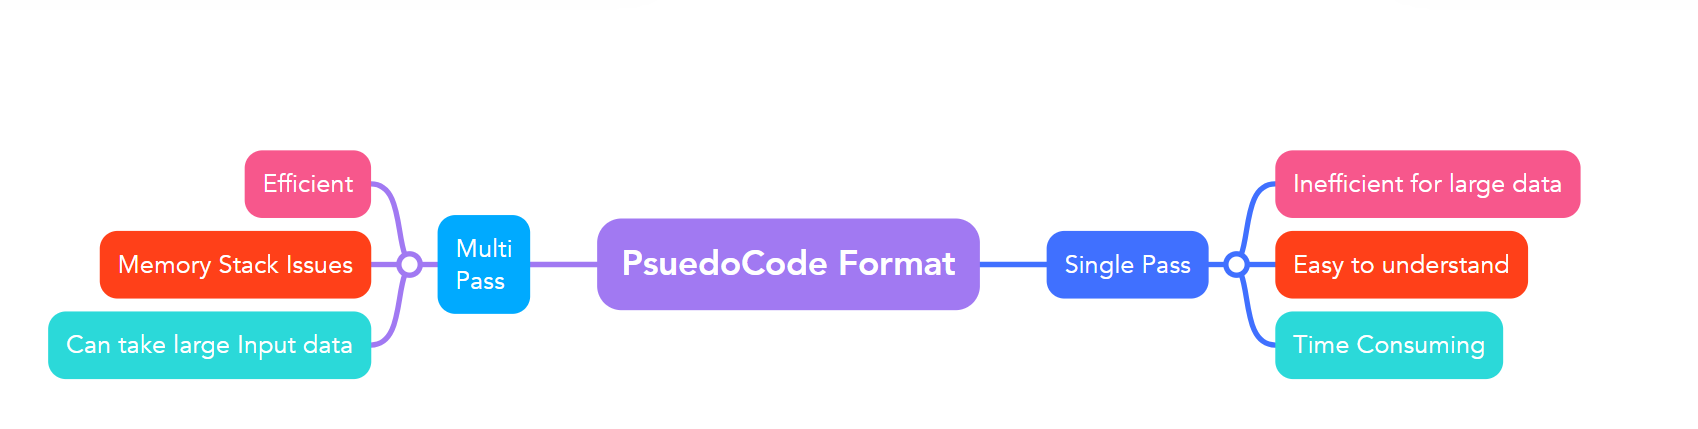
\includegraphics[width=15cm, height=10cm]{images/Mind Map.png} 
  \end{center}
  \caption{\vspace{0.8 cm}Mind Map for psuedo code format}
\end{figure}


\pagebreak

\subsection{\Large \vspace{0.2 cm}Psuedo-Code}There are two algorithms for which the psuedo code is provided below:-

\begin{algorithm}
\caption{Multi Pass Algorithm for calculating Standard Deviation}

\small
\begin{algorithmic}

\Function{StandardDeviation}{numArray[]}
\State $Sum \gets 0.0$

\State $Mean \gets 0.0$
\State $SD1 \gets 0.0$
\State $iLength \gets numArray.count()$
\For{$i = 0$ \textbf{to} $iLength$}
    \State Sum = Sum + numArray[i]
\EndFor    
\State $Mean= Sum/iLength$    
\For{$i = 0$ \textbf{to} $iLength$}
    \State diff = numArray[i]-Mean
    \State SD1 =SD1 + (diff*diff)
\EndFor
return SquareRoot(SD1 /iLength)
\EndFunction


\\
\Function{SquareRoot}{input}
\State $error \gets 0.00001$
\State $errorPrecision \gets 1$
\State $dup \gets input$
\State $iLength \gets numArray.count()$
\While{$errorPrecision > error$}
   \State $input = (input+dup/input)/2$
   \State $errorPrecision = input-dup/input$
\EndWhile
return input
\EndFunction
\\

\end{algorithmic}
\end{algorithm}
\pagebreak
\begin{algorithm}
\caption{Single Pass Algorithm for calculating Standard Deviation}


\begin{algorithmic}

\Function{StandardDeviation}{numArray[]}
\State $Sum \gets 0.0$

\State $Mean \gets 0.0$
\State $SD1 \gets 0.0$
\State $iLength \gets numArray.count()$
\For{$i = 0$ \textbf{to} $iLength$}
    \State Sum = Sum + numArray[i]
    \State SqSum = SqSum + (numArray[i]*numArray[i])
\EndFor    
\State $Mean= Sum/iLength$    
\State $Variance = SqSum/n - Mean*Mean$
\\
\quad\, return SquareRoot(SD1 /iLength)
\EndFunction


\\
\Function{SquareRoot}{input}
\State $error \gets 0.00001$
\State $errorPrecision \gets 1$
\State $dup \gets input$
\State $iLength \gets numArray.count()$
\While{$errorPrecision > error$}
   \State $input = (input+dup/input)/2$
   \State $errorPrecision = input-dup/input$
\EndWhile
return input
\EndFunction
\\

\end{algorithmic}
\end{algorithm}


\begin{thebibliography}{9}
\bibitem{Peter Kankowski}
Peter Kankowski
\\\texttt{https://www.strchr.com/standard\_deviation\_in\_one\_pass?allcomments=1}

\bibitem{Standard Deviations and Standard Errors} 
Standard Deviations and Standard Errors,
\\\texttt{https://www.ncbi.nlm.nih.gov/pmc/articles/PMC1255808/}


\end{thebibliography}



\end{document}